
\documentclass[border=8pt, multi, tikz]{standalone} 
\usepackage{import}
\subimport{../layers/}{init}
\usetikzlibrary{positioning}
\usetikzlibrary{3d} %for including external image 

\def\ConvColor{rgb:yellow,5;red,2.5;white,5}
\def\ConvReluColor{rgb:yellow,5;red,5;white,5}
\def\PoolColor{rgb:red,1;black,0.3}
\def\UnpoolColor{rgb:blue,2;green,1;black,0.3}
\def\FcColor{rgb:blue,5;red,2.5;white,5}
\def\FcReluColor{rgb:blue,5;red,5;white,4}
\def\SoftmaxColor{rgb:magenta,5;black,7}
\def\DropColor{rgb:blue,5;red,2.5;white,5}

\newcommand{\copymidarrow}{\tikz \draw[-Stealth,line width=0.8mm,draw={rgb:blue,4;red,1;green,1;black,3}] (-0.3,0) -- ++(0.3,0);}

\begin{document}
\begin{tikzpicture}
\tikzstyle{connection}=[ultra thick,every node/.style={sloped,allow upside down},draw=\edgecolor,opacity=0.7]
\tikzstyle{copyconnection}=[ultra thick,every node/.style={sloped,allow upside down},draw={rgb:blue,4;red,1;green,1;black,3},opacity=0.7]

\node[canvas is zy plane at x=0] (temp) at (-3,0,0) {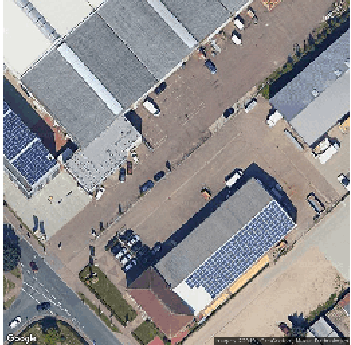
\includegraphics[width=8cm,height=8cm]{data/input.PNG}};

\pic[shift={ (-2,0,0) }] at (0,0,0) 
    {RightBandedBox={
        name=ccr_b0,
        caption= ,
        xlabel={{ ,  }},
        zlabel=,
        fill=\ConvColor,
        bandfill=\ConvReluColor,
        height=35,
        width={ 1 , 1 },
        depth=35
        }
    };

\pic[shift={ (-1,0,0) }] at (ccr_b1-east) 
    {Box={
        name=pool_b1,
        caption=Pooling,
        fill=\PoolColor,
        opacity=0.5,
        height=35,
        width=1,
        depth=35
        }
    };

\pic[shift={ (0,0,0) }] at (0,0,0) 
    {RightBandedBox={
        name=ccr_b1,
        caption= ,
        xlabel={{ ,   ,  }},
        zlabel=,
        fill=\ConvColor,
        bandfill=\ConvReluColor,
        height=32,
        width={ 1 , 1, 1 },
        depth=32
        }
    };

\pic[shift={ (1,0,0) }] at (ccr_b1-east) 
    {RightBandedBox={
        name=ccr_b2,
        caption= ,
        xlabel={{ ,  ... ,  }},
        zlabel=,
        fill=\ConvColor,
        bandfill=\ConvReluColor,
        height=28,
        width={ 2.5 , 2.5, 2.5 },
        depth=28
        }
    };

\draw [connection]  (ccr_b1-east)    -- node {\midarrow} (ccr_b2-west);

\pic[shift={ (1,0,0) }] at (ccr_b2-east) 
    {RightBandedBox={
        name=ccr_b3,
        caption= ,
        xlabel={{ ,  ... ,  }},
        zlabel=,
        fill=\ConvColor,
        bandfill=\ConvReluColor,
        height=25,
        width={ 3.5 , 3.5, 3.5 },
        depth=25
        }
    };

\draw [connection]  (ccr_b2-east)    -- node {\midarrow} (ccr_b3-west);

\pic[shift={ (1,0,0) }] at (ccr_b3-east) 
    {RightBandedBox={
        name=ccr_b4,
        caption= ,
        xlabel={{ ,  ... ,  }},
        zlabel=,
        fill=\ConvColor,
        bandfill=\ConvReluColor,
        height=16,
        width={ 4.5 , 4.5, 4.5 },
        depth=16
        }
    };

\draw [connection]  (ccr_b3-east)    -- node {\midarrow} (ccr_b4-west);

\pic[shift={(2,0,0)}] at (ccr_b4-east) 
    {Box={
        name=ccr_resbottle,
        caption=,
        xlabel={{ , }},
        zlabel=,
        fill=\ConvColor,
        height=8,
        width=8,
        depth=8
        }
    };

\pic[shift={(0,0,0)}] at (ccr_resbottle-east) 
    {Box={
        name=ccr_drop_cbottle,
        caption=Dropout,
        xlabel={{" ", " "}},
        zlabel=,
        fill=\DropColor,
        height=8,
        width=2,
        depth=8
        }
    };

\pic[shift={(0,0,0)}] at (ccr_drop_cbottle-east) 
    {Box={
        name=ccr_bottle,
        caption=,
        xlabel={{ , }},
        zlabel=,
        fill=\ConvColor,
        height=8,
        width=8,
        depth=8
        }
    };

\draw [connection]  (ccr_b4-east)    -- node {\midarrow} (ccr_resbottle-west);

\pic[shift={ (1,0,0) }] at (ccr_bottle-east) 
    {RightBandedBox={
        name=ccr_b6,
        caption= ,
        xlabel={{ ,  ... ,  }},
        zlabel=,
        fill=\ConvColor,
        bandfill=\ConvReluColor,
        height=16,
        width={ 4.5 , 4.5, 4.5 },
        depth=16
        }
    };

\draw [connection]  (ccr_bottle-east)    -- node {\midarrow} (ccr_b6-west);

\path (ccr_b4-southeast) -- (ccr_b4-northeast) coordinate[pos=1.25] (ccr_b4-top) ;
\path (ccr_b6-south)  -- (ccr_b6-north)  coordinate[pos=1.25] (ccr_b6-top) ;
\draw [copyconnection]  (ccr_b4-northeast)  
-- node {\copymidarrow}(ccr_b4-top)
-- node {\copymidarrow}(ccr_b6-top)
-- node {\copymidarrow} (ccr_b6-north);

\pic[shift={ (1,0,0) }] at (ccr_b6-east) 
    {RightBandedBox={
        name=ccr_b7,
        caption= ,
        xlabel={{ ,  ... ,  }},
        zlabel=,
        fill=\ConvColor,
        bandfill=\ConvReluColor,
        height=25,
        width={ 3.5 , 3.5, 3.5 },
        depth=25
        }
    };

\draw [connection]  (ccr_b6-east)    -- node {\midarrow} (ccr_b7-west);

\path (ccr_b3-southeast) -- (ccr_b3-northeast) coordinate[pos=1.25] (ccr_b3-top) ;
\path (ccr_b7-south)  -- (ccr_b7-north)  coordinate[pos=1.25] (ccr_b7-top) ;
\draw [copyconnection]  (ccr_b3-northeast)  
-- node {\copymidarrow}(ccr_b3-top)
-- node {\copymidarrow}(ccr_b7-top)
-- node {\copymidarrow} (ccr_b7-north);

\pic[shift={ (1,0,0) }] at (ccr_b7-east) 
    {RightBandedBox={
        name=ccr_b8,
        caption= ,
        xlabel={{ ,  ... ,  }},
        zlabel=,
        fill=\ConvColor,
        bandfill=\ConvReluColor,
        height=28,
        width={ 2.5 , 2.5, 2.5 },
        depth=28
        }
    };

\draw [connection]  (ccr_b7-east)    -- node {\midarrow} (ccr_b8-west);

\path (ccr_b2-southeast) -- (ccr_b2-northeast) coordinate[pos=1.25] (ccr_b2-top) ;
\path (ccr_b8-south)  -- (ccr_b8-north)  coordinate[pos=1.25] (ccr_b8-top) ;
\draw [copyconnection]  (ccr_b2-northeast)  
-- node {\copymidarrow}(ccr_b2-top)
-- node {\copymidarrow}(ccr_b8-top)
-- node {\copymidarrow} (ccr_b8-north);

\pic[shift={ (1,0,0) }] at (ccr_b8-east) 
    {RightBandedBox={
        name=ccr_b9,
        caption= ,
        xlabel={{ ,  ... ,  }},
        zlabel=,
        fill=\ConvColor,
        bandfill=\ConvReluColor,
        height=32,
        width={ 1 , 1, 1 },
        depth=32
        }
    };

\draw [connection]  (ccr_b8-east)    -- node {\midarrow} (ccr_b9-west);

\path (ccr_b1-southeast) -- (ccr_b1-northeast) coordinate[pos=1.25] (ccr_b1-top) ;
\path (ccr_b9-south)  -- (ccr_b9-north)  coordinate[pos=1.25] (ccr_b9-top) ;
\draw [copyconnection]  (ccr_b1-northeast)  
-- node {\copymidarrow}(ccr_b1-top)
-- node {\copymidarrow}(ccr_b9-top)
-- node {\copymidarrow} (ccr_b9-north);

\pic[shift={(0.75,0,0)}] at (ccr_b9-east) 
    {Box={
        name=soft1,
        caption=SIGMOID,
        zlabel=,
        fill=\SoftmaxColor,
        height=40,
        width=1,
        depth=40
        }
    };

\draw [connection]  (ccr_b9-east)    -- node {\midarrow} (soft1-west);

\draw [connection]  (ccr_b9-east)    -- node {\midarrow} (soft1-west);
 
    \node[canvas is zy plane at x=3] (temp) at (soft1-east) {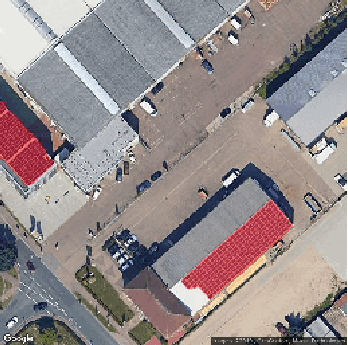
\includegraphics[width=8cm,height=8cm]{data/output.PNG}}; 

\end{tikzpicture}
\end{document}
